\documentclass[11pt]{article}

\usepackage{graphicx}
\usepackage{multirow}
\usepackage{fullpage}
\usepackage{mathtools}
\usepackage{kbordermatrix}
\usepackage{amsmath,amsfonts,amssymb}
\usepackage{blkarray}
\usepackage{listings}
\lstset{language=MATLAB}%Program language is MATLAB
\lstset{breaklines}%Wrap longline automatically
\lstset{extendedchars=false}



\begin{document}
\tableofcontents

\title{ECE595 Project 1 Report}
\author{Niu,Wensen and Shen,Dan}
\date{\today}
\maketitle
\begin{flushleft}
\section{About This Project}
	Firstly, we recall the problem and tasks of this project in this chapter. Instantaneously, we introduce what we did for this project.
	\subsection{Conditions}
	"Cat and Mouse" problem is a typical problem of mutual exclusion problem which can be solved by the application of petri net. In this project, we consider that there are 4 rooms in a house and the house layout is shown as Figure 1.
	\begin{center}
	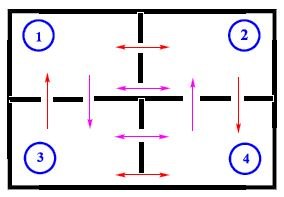
\includegraphics[]{houselayout.JPG}
	
	Figure 1 House layout
	\end{center}
	The cat can move following the direction of red arrows. And the mouse can move following the direction of purple arrows. Initially, the cat is in Room 4 and the mouse is in Room 1.
	
	\subsection{Tasks}
	1. Build a Petri net model for the movement of the cat;
	
	2. Build a petri net model for the movement of the mouse;
	
	3. Design a Petri net controller to guarantee that the cat and mouse can never be in the same room.
	
	4. Write a computer program (preferably in MATLAB or C) to calculate all possible reachable states of the Controlled Petri net.
		
\section{Build Petri Net Model}
	To apply the Petri net on this kind "Cat and Mouse" problem, we built Petri net model for the movement. In this Chapter, we build Petri net for the movement of the cat, build Petri net for the movement of the mouse, and design a Petri net controller for this problem to guarantee that the cat and mouse can never be in the same room as the initial state, cat is in room 4 and mouse is in room 1.
	
	\subsection{Petri net model for the movement of the cat}
	Firstly, for building Petri net model for the movement of the cat, we build place set, transition set and arcs set:
	
	Place set: $$P_{cat}=\{P_{cat1},\ P_{cat2},\ P_{cat3},\ P_{cat4}\};$$
	
	Transition set: $$T_{cat}=\{t_{12C},\ t_{21C},\ t_{24},\ t_{31},\  t_{34C},\ t_{43C}\};$$
	
	Arcs set: $A_{cat}=$
	\begin{equation*}
	\begin{array}{*{4}c}
	\{(P_{cat1},\ t_{12C}), & (t_{12C},\ P_{cat2}), & (P_{cat2},\ t_{21C}), & (t_{21C},\ P_{cat1}),\\
	\ (P_{cat2}, t_{24}), & (t_{24},\ P_{cat2}), & (P_{cat3},\ t_{31C}), & (t_{31C},\ P_{cat1}),\\
	\ (P_{cat3},\ t_{34C}), & (t_{34C},\ P_{cat4}), & (P_{cat4},\ t_{43C}), & (t_{43C},\ P_{cat3})\}.
	\end{array}
	\end{equation*}
	
%	\begin{equation*}
%	\begin{array}{*{4}c}
%	\{(P_{mouse1},\ t_{12M}), & (t_{12M},\ P_{mouse2}), & (P_{mouse2},\ t_{21M}), & (t_{21M},\ P_{mouse1}),\\
%	(P_{mouse1}, t_{13}), & (t_{13},\ P_{mouse3}), & (P_{mouse3},\ t_{34M}), & (t_{34M},\ P_{mouse4}),\\
%	(P_{mouse4},\ t_{43M}), & (t_{43M},\ P_{mouse3}), & (P_{mouse4},\ t_{42M}), & (t_{42M},\ P_{mouse2})
%	\}
%	\end{array}
%	\end{equation*}
	
%	\begin{center}
%	$A_{cat}=\{(P_{cat1},\ t_{12C}),\ (t_{12C},\ P_{cat2}),\ (P_{cat2},\ t_{21C}),\ (t_{21C},\ P_{cat1}),$
%	$\ (P_{cat2}, t_{24}),\ (t_{24},\ P_{cat2}),\ (P_{cat3},\ t_{31C}),\ (t_{31C},\ P_{cat1}),$
%	$\ (P_{cat3},\ t_{34C}),\ (t_{34C},\ P_{cat4}),\ (P_{cat4},\ t_{43C}),\ (t_{43C},\ P_{cat3})\}$.
%	\end{center}
	Secondly, we calculate incident matrix of this Petri net. This Petri net has 4 places, 6 transitions. We can unique define input incident matrix $B_{Cat}^-$, captures are weights from places to transitions. The dimension of input incident matrix is $4\times 6$.
	
	The weights from places to transitions are:
	
	\begin{center}
	\begin{tabular}{ccccccc}

	& $t_{12C}$ & $t_{21C}$ & $t_{24}$ & $t_{31}$ & $t_{34C}$ & $t_{43C}$\\
	$P_{cat1}$ & 1 & 0 & 0 & 0 & 0 & 0\\
	$P_{cat2}$ & 0 & 1 & 1 & 0 & 0 & 0\\
	$P_{cat3}$ & 0 & 0 & 0 & 1 & 1 & 0\\
	$P_{cat4}$ & 0 & 0 & 0 & 0 & 0 & 1\\
	\end{tabular}
	\end{center}
	
	Input incident matrix is:
	\begin{equation*}
	B_{Cat}^-=
	\kbordermatrix{
	& t_{12C} & t_{21C} & t_{24} & t_{31} & t_{34C} & t_{43C}\cr
	P_{cat1} & 1 & 0 & 0 & 0 & 0 & 0\cr
	P_{cat2} & 0 & 1 & 1 & 0 & 0 & 0\cr
	P_{cat3} & 0 & 0 & 0 & 1 & 1 & 0\cr
	P_{cat4} & 0 & 0 & 0 & 0 & 0 & 1\cr
	}	
	\end{equation*}

%	\begin{equation*}
%	\left[
%	\begin{array}{cccccc}
%	1 & 0 & 0 & 0 & 0 & 0\\
%	0 & 1 & 1 & 0 & 0 & 0\\
%	0 & 0 & 0 & 1 & 1 & 0\\
%	0 & 0 & 0 & 0 & 0 & 1\\
%    \end{array}
%    \right]
%    \end{equation*}
        
    Also, we can unique define output incident matrix $B_{Cat}^+$, captures are weights from transitions to places. The dimension of output incident matrix is $4\times 6$.
    
    The weights from transitions to places are:
    
	\begin{center}
	\begin{tabular}{ccccccc}
	& $t_{12C}$ & $t_{21C}$ & $t_{24}$ & $t_{31}$ & $t_{34C}$ & $t_{43C}$\\
	$P_{cat1}$ & 0 & 1 & 0 & 1 & 0 & 0\\
	$P_{cat2}$ & 1 & 0 & 0 & 0 & 0 & 0\\
	$P_{cat3}$ & 0 & 0 & 0 & 0 & 0 & 1\\
	$P_{cat4}$ & 0 & 0 & 1 & 0 & 1 & 0\\
	\end{tabular}
	\end{center}
	
    The output incident matrix is: 
    \begin{equation*}
    B_{Cat}^+=
    \kbordermatrix{
    & t_{12C} & t_{21C} & t_{24} & t_{31} & t_{34C} & t_{43C}\cr
	P_{cat1} & 0 & 1 & 0 & 1 & 0 & 0\cr
	P_{cat2} & 1 & 0 & 0 & 0 & 0 & 0\cr
	P_{cat3} & 0 & 0 & 0 & 0 & 0 & 1\cr
	P_{cat4} & 0 & 0 & 1 & 0 & 1 & 0\cr
    }
    \end{equation*}

%	\begin{equation*}
%	\left[
%	\begin{array}{cccccc}
%	0 & 1 & 0 & 1 & 0 & 0\\
%	1 & 0 & 0 & 0 & 0 & 0\\
%	0 & 0 & 0 & 0 & 0 & 1\\
%	0 & 0 & 1 & 0 & 1 & 0\\
%    \end{array}
%    \right]
%    \end{equation*}
    
    The incident matrix is: 
    \begin{equation*}
    B_{Cat}= B_{Cat}^+-B_{Cat}^-=
	\kbordermatrix{
	& t_{12C} & t_{21C} & t_{24} & t_{31} & t_{34C} & t_{43C}\cr
	P_{cat1} & -1 & 1 & 0 & 1 & 0 & 0\cr
	P_{cat2} & 1 & -1 & -1 & 0 & 0 & 0\cr
	P_{cat3} & 0 & 0 & 0 & -1 & -1 & 1\cr
	P_{cat4} & 0 & 0 & 1 & 0 & 1 & -1\cr
	}
    \end{equation*}
    
    The Petri net graph for the Petri net model for movement of cat is shown as Figure 2.
    \begin{center}
	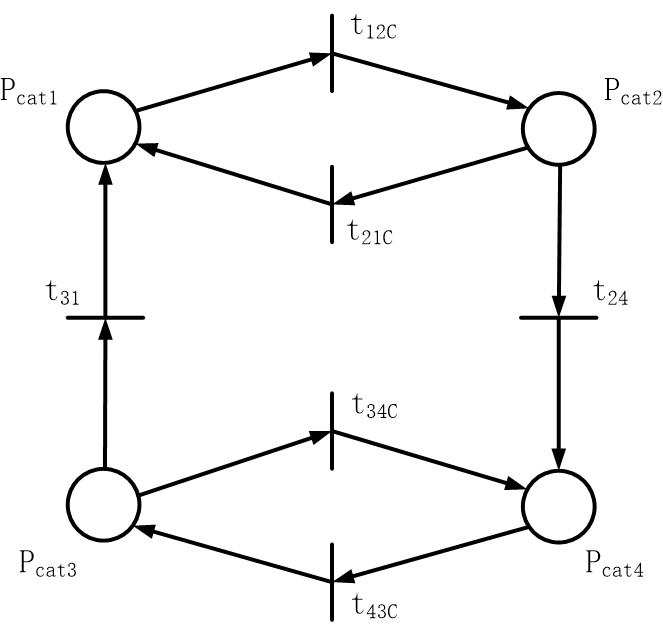
\includegraphics[width=12cm,height=10cm]{movementofcat.JPG}
	
	Figure 2 Petri net graph for movement of cat.
	\end{center}
    
	\newpage
	\subsection{Petri net model for the movement of the mouse}
	Same as we built place set, transition set, and arcs set for building Petri net model for the movement of cat. For building the petri net model for movement of mouse, we also build place set, transition set and arcs set at first:
	
	Place set: $$P_{mouse}=\{P_{mouse1},\ P_{mouse2},\ P_{mouse3},\ P_{mouse4}\};$$
	
	Transition set: $$T_{mouse}=\{t_{12M},\ t_{21M},\ t_{13},\ t_{34M},\  t_{43M},\ t_{42}\};$$
	
	Arcs set: 
	$A_{mouse}=$
	\begin{equation*}
	\begin{array}{*{4}c}
	\{(P_{mouse1},\ t_{12M}), & (t_{12M},\ P_{mouse2}), & (P_{mouse2},\ t_{21M}), & (t_{21M},\ P_{mouse1}),\\
	(P_{mouse1}, t_{13}), & (t_{13},\ P_{mouse3}), & (P_{mouse3},\ t_{34M}), & (t_{34M},\ P_{mouse4}),\\
	(P_{mouse4},\ t_{43M}), & (t_{43M},\ P_{mouse3}), & (P_{mouse4},\ t_{42M}), & (t_{42M},\ P_{mouse2})\}.
	\end{array}
	\end{equation*}
%	\begin{center}
%	$A_{mouse}=\{(P_{mouse1},\ t_{12M}),\ (t_{12M},\ P_{mouse2}),\ (P_{mouse2},\ t_{21M}),\ (t_{21M},\ P_{mouse1}),$
%	$\ (P_{mouse1}, t_{13}),\ (t_{13},\ P_{mouse3}),\ (P_{mouse3},\ t_{34M}),\ (t_{34M},\ P_{mouse4}),$
%	$\ (P_{mouse4},\ t_{43M}),\ (t_{43M},\ P_{mouse3}),\ (P_{mouse4},\ t_{42M}),\ (t_{42M},\ P_{mouse2})\}$.
%	\end{center}
	And then, we calculate incident matrix of this Petri net model for movement of mouse. It also has 4 places and 6 transitions. The unique input incident matrix $B_{Mouse}^-$, captures are weights from places to transitions with $4\times 6$ dimension. And the output incident matrix $B_{Mouse}^+$, captures are weights from transitions to places with $4\times 6$ dimension.
	
	The weights from places to transitions of the Petri net for movement of mouse are:
	
	\begin{center}
	\begin{tabular}{ccccccc}

	& $t_{12M}$ & $t_{21M}$ & $t_{13}$ & $t_{34M}$ & $t_{43M}$ & $t_{42}$\\
	$P_{mouse1}$ & 1 & 0 & 1 & 0 & 0 & 0\\
	$P_{mouse2}$ & 0 & 1 & 0 & 0 & 0 & 0\\
	$P_{mouse3}$ & 0 & 0 & 0 & 1 & 0 & 0\\
	$P_{mouse4}$ & 0 & 0 & 0 & 0 & 1 & 1\\
	\end{tabular}
	\end{center}
	
	Input incident matrix is: 
	\begin{equation*}
	B_{Mouse}^-=
	\kbordermatrix{
	& t_{12M} & t_{21M} & t_{13} & t_{34M} & t_{43M} & t_{42}\cr
	P_{mouse1} & 1 & 0 & 1 & 0 & 0 & 0\cr
	P_{mouse2} & 0 & 1 & 0 & 0 & 0 & 0\cr
	P_{mouse3} & 0 & 0 & 0 & 1 & 0 & 0\cr
	P_{mouse4} & 0 & 0 & 0 & 0 & 1 & 1
	}
	\end{equation*}
%	
%	\begin{equation*}
%	\left[
%	\begin{array}{cccccc}
%	1 & 0 & 1 & 0 & 0 & 0\\
%	0 & 1 & 0 & 0 & 0 & 0\\
%	0 & 0 & 0 & 1 & 0 & 0\\
%	0 & 0 & 0 & 0 & 1 & 1\\
%    \end{array}
%    \right]
%    \end{equation*}
        
    
    
    The weights from transitions to places are:
    
	\begin{center}
	\begin{tabular}{ccccccc}
	& $t_{12M}$ & $t_{21M}$ & $t_{13}$ & $t_{34M}$ & $t_{43M}$ & $t_{42}$\\
	$P_{mouse1}$ & 0 & 1 & 0 & 0 & 0 & 0\\
	$P_{mouse2}$ & 1 & 0 & 0 & 0 & 0 & 1\\
	$P_{mouse3}$ & 0 & 0 & 1 & 0 & 1 & 0\\
	$P_{mouse4}$ & 0 & 0 & 0 & 1 & 0 & 0\\
	\end{tabular}
	\end{center}
	
    output incident matrix is: 
	\begin{equation*}
	B_{Mouse}^+=
	\kbordermatrix{
	& t_{12M} & t_{21M} & t_{13} & t_{34M} & t_{43M} & t_{42}\cr
	P_{mouse1} & 0 & 1 & 0 & 0 & 0 & 0\cr
	P_{mouse2} & 1 & 0 & 0 & 0 & 0 & 1\cr
	P_{mouse3} & 0 & 0 & 1 & 0 & 1 & 0\cr
	P_{mouse4} & 0 & 0 & 0 & 1 & 0 & 0\cr
	}   
    \end{equation*}
    
    The incident matrix is:
    \begin{equation*}
    B_{Mouse}= B_{Mouse}^+-B_{Mouse}^-=
	\kbordermatrix{
	& t_{12M} & t_{21M} & t_{13} & t_{34M} & t_{43M} & t_{42}\\
	P_{mouse1} & -1 & 1 & -1 & 0 & 0 & 0\\
	P_{mouse2} & 1 & -1 & 0 & 0 & 0 & 1\\
	P_{mouse3} & 0 & 0 & 1 & -1 & 1 & 0\\
	P_{mouse4} & 0 & 0 & 0 & 1 & -1 & -1\\
	}
    \end{equation*}
    
    The Petri net graph for this Petri net model is shown as Figure 3.
    \begin{center}
	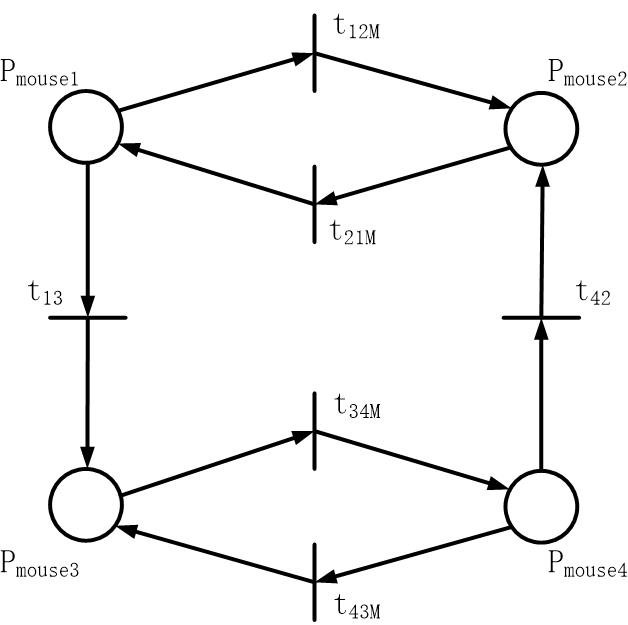
\includegraphics[width=12cm,height=10cm]{movementofmouse.JPG}
	
	Figure 3 Petri net graph for movement of mouse.
	\end{center}
	
	\newpage
	\subsection{Design a Petri net controller}
	
	In this part, we design a Petri net controller to guarantee that cat and mouse can never be in the same room with that initially the cat is in Room 4 and the mouse is in Room 1. We combine the Petri net model for the movement of cat and mouse to build a Petri net for this "Cat and Mouse" problem. After combined, the place set, transition set, and arc set of the new Petri net is:
	
	Place set:$$P=\{P_{cat1},\ P_{cat2},\ P_{cat3},\ P_{cat4},\ P_{mouse1},\ P_{mouse2},\ P_{mouse3},\ P_{mouse4}\};$$
	
	Transition set:$$T=\{t_{12C},\ t_{21C},\ t_{24},\ t_{31},\  t_{34C},\ t_{43C},\ t_{12M},\ t_{21M},\ t_{13},\ t_{34M},\  t_{43M},\ t_{42}\};$$
	
	Arc set: $A=$
	\begin{equation*}
	\begin{array}{*{4}c}
	\{(P_{cat1},\ t_{12C}), & (t_{12C},\ P_{cat2}), & (P_{cat2},\ t_{21C}), & (t_{21C},\ P_{cat1}),\\
	\ (P_{cat2}, t_{24}), & (t_{24},\ P_{cat2}), & (P_{cat3},\ t_{31C}), & (t_{31C},\ P_{cat1}),\\
	\ (P_{cat3},\ t_{34C}), & (t_{34C},\ P_{cat4}), & (P_{cat4},\ t_{43C}), & (t_{43C},\ P_{cat3})\\
	\ (P_{mouse1},\ t_{12M}), & (t_{12M},\ P_{mouse2}), & (P_{mouse2},\ t_{21M}), & (t_{21M},\ P_{mouse1}),\\
	\ (P_{mouse1}, t_{13}), & (t_{13},\ P_{mouse3}), & (P_{mouse3},\ t_{34M}), & (t_{34M},\ P_{mouse4}),\\
	\ (P_{mouse4},\ t_{43M}), & (t_{43M},\ P_{mouse3}), & (P_{mouse4},\ t_{42M}), & (t_{42M},\ P_{mouse2})\}.
	\end{array}
	\end{equation*}	
%	$A_{mouse}=$
%	\begin{equation*}
%	\begin{array}{*{4}c}
%	\{(P_{mouse1},\ t_{12M}), & (t_{12M},\ P_{mouse2}), & (P_{mouse2},\ t_{21M}), & (t_{21M},\ P_{mouse1}),\\
%	(P_{mouse1}, t_{13}), & (t_{13},\ P_{mouse3}), & (P_{mouse3},\ t_{34M}), & (t_{34M},\ P_{mouse4}),\\
%	(P_{mouse4},\ t_{43M}), & (t_{43M},\ P_{mouse3}), & (P_{mouse4},\ t_{42M}), & (t_{42M},\ P_{mouse2})
%	\}
%	\end{array}
%	\end{equation*}
%	\begin{center}
%	$A=\{(P_{cat1},\ t_{12C}),\ (t_{12C},\ P_{cat2}),\ (P_{cat2},\ t_{21C}),\ (t_{21C},\ P_{cat1}),$
%	
%	$\ (P_{cat2}, t_{24}),\ (t_{24},\ P_{cat2}),\ (P_{cat3},\ t_{31C}),\ (t_{31C},\ P_{cat1}),$
%
%	$\ (P_{cat3},\ t_{34C}),\ (t_{34C},\ P_{cat4}),\ (P_{cat4},\ t_{43C}),\ (t_{43C},\ P_{cat3})$
%
%	$(P_{mouse1},\ t_{12M}),\ (t_{12M},\ P_{mouse2}),\ (P_{mouse2},\ t_{21M}),\ (t_{21M},\ P_{mouse1}),$
%
%	$\ (P_{mouse1}, t_{13}),\ (t_{13},\ P_{mouse3}),\ (P_{mouse3},\ t_{34M}),\ (t_{34M},\ P_{mouse4}),$
%
%	$\ (P_{mouse4},\ t_{43M}),\ (t_{43M},\ P_{mouse3}),\ (P_{mouse4},\ t_{42M}),\ (t_{42M},\ P_{mouse2})\}$.
%	\end{center}
The input incident matrix is:
	\begin{equation*}
	B^-=
	\kbordermatrix{
	&t_{12C}&t_{21C}&t_{24}&t_{31}&t_{34C}&t_{43C}&t_{12C}&t_{21C}&t_{24}&t_{31}&t_{34C}&t_{43C}\\
	P_{cat1}&1&0&0&0&0&0&0&0&0&0&0&0\\
	P_{cat2}&0&1&1&0&0&0&0&0&0&0&0&0\\
	P_{cat3}&0&0&0&1&1&0&0&0&0&0&0&0\\
	P_{cat4}&0&0&0&0&0&1&0&0&0&0&0&0\\
	P_{mouse1}&0&0&0&0&0&0&1&0&1&0&0&0\\
	P_{mouse2}&0&0&0&0&0&0&0&1&0&0&0&0\\
	P_{mouse3}&0&0&0&0&0&0&0&0&0&1&0&0\\
	P_{mouse4}&0&0&0&0&0&0&0&0&0&0&1&1\\
	}
	\end{equation*}
	The output incident matrix is:
	\begin{equation*}
	B^+=
	\kbordermatrix{
	&t_{12C}&t_{21C}&t_{24}&t_{31}&t_{34C}&t_{43C}&t_{12C}&t_{21C}&t_{24}&t_{31}&t_{34C}&t_{43C}\\
	P_{cat1}&0&1&0&1&0&0&0&0&0&0&0&0\\
	P_{cat2}&1&0&0&0&0&0&0&0&0&0&0&0\\
	P_{cat3}&0&0&0&0&0&1&0&0&0&0&0&0\\
	P_{cat4}&0&0&1&0&1&0&0&0&0&0&0&0\\
	P_{mouse1}&0&0&0&0&0&0&0&1&0&0&0&0\\
	P_{mouse2}&0&0&0&0&0&0&1&0&0&0&0&1\\
	P_{mouse3}&0&0&0&0&0&0&0&0&1&0&1&0\\
	P_{mouse4}&0&0&0&0&0&0&0&0&0&1&0&0\\
	}
	\end{equation*}
Because of that cat is in Room 4 and mouse is in Room 1 initially, the initial state of this Petri net is:
	\begin{equation*}
	M_0^\top=
	\kbordermatrix{
	& P_{cat1} & P_{cat2} & P_{cat3} & P_{cat4} & P_{mouse1} & P_{mouse2} & P_{mouse3} & P_{mouse4}\cr
	& 0 & 0 & 0 & 1 & 1 & 0 & 0 & 0\cr
	}
	\end{equation*}
we transfer the constraint to the form:$$LM\leq b,$$
Where 
	\begin{equation*}
	L=
	\kbordermatrix{
	\\
	& 1 & 0 & 0 & 0 & 1 & 0 & 0 & 0\\
	& 0 & 1 & 0 & 0 & 0 & 1 & 0 & 0\\
	& 0 & 0 & 1 & 0 & 0 & 0 & 1 & 0\\
	& 0 & 0 & 0 & 1 & 0 & 0 & 0 & 1\\
	},\  
	\ M=
	\kbordermatrix{
	\\
	&M(P_{cat1})\\
	&M(P_{cat2})\\
	&M(P_{cat3})\\
	&M(P_{cat4})\\
	&M(P_{mouse1})\\
	&M(P_{mouse2})\\
	&M(P_{mouse3})\\
	&M(P_{mouse4})\\
	},\ 	
	\ b=
	\kbordermatrix{
	\\
	&1\\
	&1\\
	&1\\
	&1\\
	}
	\end{equation*}
%	\begin{equation*}
%	
%	\end{equation*}
	According to the input incident matrix and output incident matrix, the incident matrix is:
	\begin{equation*}
	B=B^+-B^-=
	\kbordermatrix{
	&t_{12C}&t_{21C}&t_{24}&t_{31}&t_{34C}&t_{43C}&t_{12C}&t_{21C}&t_{24}&t_{31}&t_{34C}&t_{43C}\\
	P_{cat1}&-1&1&0&1&0&0&0&0&0&0&0&0\\
	P_{cat2}&1&-1&-1&0&0&0&0&0&0&0&0&0\\
	P_{cat3}&0&0&0&-1&-1&1&0&0&0&0&0&0\\
	P_{cat4}&0&0&1&0&1&-1&0&0&0&0&0&0\\
	P_{mouse1}&0&0&0&0&0&0&-1&1&-1&0&0&0\\
	P_{mouse2}&0&0&0&0&0&0&1&-1&0&0&0&1\\
	P_{mouse3}&0&0&0&0&0&0&0&0&1&-1&1&0\\
	P_{mouse4}&0&0&0&0&0&0&0&0&0&1&-1&-1\\
	}	
	\end{equation*}
For $LM\leq b$, we introduce a slack variable, $M_c$, the state of the controller($M_c\geq 0$). Such that $$LM+M_c=b$$
\[
\left[\begin{array}{c|c}
L &I
\end{array}\right]
\left[\begin{array}{c}
M\\
\hline
M_c\\
\end{array}
\right]=b
\]
Use place invariant to design controller:

Based on the definition of place invariant, we have$$X^\top B=0\ \Rightarrow\ LB+B_c=0$$
$$\Rightarrow\ B_c=0-LB=-LB$$
\begin{equation*}
B_c=
\kbordermatrix{
&t_{12C}&t_{21C}&t_{24}&t_{31}&t_{34C}&t_{43C}&t_{12C}&t_{21C}&t_{24}&t_{31}&t_{34C}&t_{43C}\\
P_{C1}&1&-1&0&-1&0&0&1&-1&1&0&0&0\\
P_{C2}&-1&1&1&0&0&0&-1&1&0&0&0&-1\\
P_{C3}&0&0&0&1&1&-1&0&0&-1&1&-1&0\\
P_{C4}&0&0&-1&0&-1&1&0&0&0&-1&1&1\\
}
\end{equation*}
The initial state of the Petri net controller is obtained by $$LM+M_c=b\ \Rightarrow \ LM_0+M_{C0}=b$$
The initial state is:
\begin{equation*}
M_{C0}=b-LM_0=
\kbordermatrix{
\\
&1\\
&1\\
&1\\
&1\\
}\ -
\kbordermatrix{
\\
&1\\
&0\\
&0\\
&1\\
}\ =
\kbordermatrix{
\\
&0\\
&1\\
&1\\
&0\\
}
\end{equation*}
The Petri net graph for "Cat and Mouse" problem with controller is shown in Figure 4.
    \begin{center}
	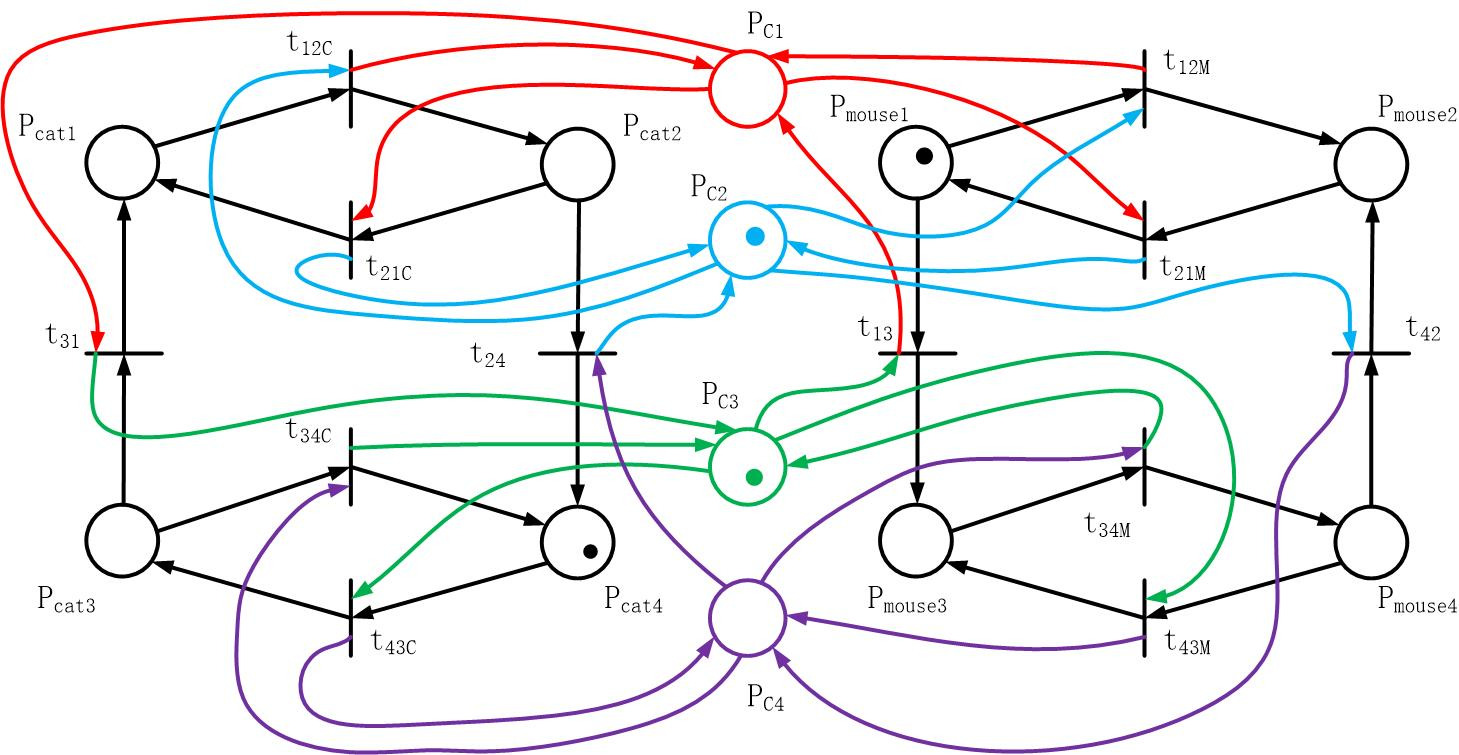
\includegraphics[width=16cm,height=12cm]{controlledpetrinetwithinitialstate.JPG}
	
	Figure 4 Petri net graph for the Petri net with controller.
	\end{center}

\newpage
\section{Computer program}
This chapter introduces a computer program designed for calculate the reachable states of a Petri net with controller. The program using MATLAB includes five functions to calculate and a m-file for input initial conditions that define the Petri net to be calculated. 

We assume that a controller need to be designed for a marked Petri net. From the definition of marked Petri net, it is a five-tuple $(P,T,A,\omega,x)$ where $(P,T,A,\omega)$ is a Petri net graph and $x$ is a marking of the set of places $P$;  $x=[x_{p1},x_{p2},...,x_{pn}]\in \mathbb{N}^n$ is the row vector associated with $x$. For programming, we treat a Petri net with constraint as a five-tuple $(B^-,B^+,L,b,M_0)$ where $B^-$ and $B^+$ is the input and output incident matrix, $M_0$ is the initial states of Petri net, and $L$ with $b$ form the constraint matrix of the Petri net which can be used to design controller as state-based controll.

For this "Cat and Mouse" problem,

The input incident matrix is:
	\begin{equation*}
	B^-=
	\kbordermatrix{
	&t_1&t_2&t_3&t_4&t_5&t_6&t_7&t_8&t_9&t_{10}&t_{11}&t_{12}\\
	P_1&1&0&0&0&0&0&0&0&0&0&0&0\\
	P_2&0&1&1&0&0&0&0&0&0&0&0&0\\
	P_3&0&0&0&1&1&0&0&0&0&0&0&0\\
	P_4&0&0&0&0&0&1&0&0&0&0&0&0\\
	P_5&0&0&0&0&0&0&1&0&1&0&0&0\\
	P_6&0&0&0&0&0&0&0&1&0&0&0&0\\
	P_7&0&0&0&0&0&0&0&0&0&1&0&0\\
	P_8&0&0&0&0&0&0&0&0&0&0&1&1\\
	}
	\end{equation*}
	The output incident matrix is:
	\begin{equation*}
	B^+=
	\kbordermatrix{
	&t_1&t_2&t_3&t_4&t_5&t_6&t_7&t_8&t_9&t_{10}&t_{11}&t_{12}\\
	P_1&0&1&0&1&0&0&0&0&0&0&0&0\\
	P_2&1&0&0&0&0&0&0&0&0&0&0&0\\
	P_3&0&0&0&0&0&1&0&0&0&0&0&0\\
	P_4&0&0&1&0&1&0&0&0&0&0&0&0\\
	P_5&0&0&0&0&0&0&0&1&0&0&0&0\\
	P_6&0&0&0&0&0&0&1&0&0&0&0&1\\
	P_7&0&0&0&0&0&0&0&0&1&0&1&0\\
	P_8&0&0&0&0&0&0&0&0&0&1&0&0\\
	}
	\end{equation*}

The constraint of this Petri net:
\begin{equation*}
	L=
	\kbordermatrix{
	\\
	& 1 & 0 & 0 & 0 & 1 & 0 & 0 & 0\\
	& 0 & 1 & 0 & 0 & 0 & 1 & 0 & 0\\
	& 0 & 0 & 1 & 0 & 0 & 0 & 1 & 0\\
	& 0 & 0 & 0 & 1 & 0 & 0 & 0 & 1\\
	},\  
	\ M=
	\kbordermatrix{
	\\
	&M(P_{1})\\
	&M(P_{2})\\
	&M(P_{3})\\
	&M(P_{4})\\
	&M(P_{5})\\
	&M(P_{6})\\
	&M(P_{7})\\
	&M(P_{8})\\
	},\ 	
	\ b=
	\kbordermatrix{
	\\
	&1\\
	&1\\
	&1\\
	&1\\
	}
	\end{equation*}
	Input all of these function as initial conditions into the section for inputting conditions of condition.m. Then it call functions to calculate initial states of controller and result in a "controlled Petri net" with satisfactory behavior as follow.
\begin{equation*}
B_c=
\kbordermatrix{
&t_{1}&t_{2}&t_{3}&t_{4}&t_{5}&t_{6}&t_{7}&t_{8}&t_{9}&t_{10}&t_{11}&t_{12}\\
P_{C1}&1&-1&0&-1&0&0&1&-1&1&0&0&0\\
P_{C2}&-1&1&1&0&0&0&-1&1&0&0&0&-1\\
P_{C3}&0&0&0&1&1&-1&0&0&-1&1&-1&0\\
P_{C4}&0&0&-1&0&-1&1&0&0&0&-1&1&1\\
}
M_{C0}=
\kbordermatrix{
\\
&0\\
&1\\
&1\\
&0\\
}
\end{equation*}
The results of "controlled Petri net" show below:
\begin{equation*}
B_{cpinput}=
\kbordermatrix{
&t_{1}&t_{2}&t_{3}&t_{4}&t_{5}&t_{6}&t_{7}&t_{8}&t_{9}&t_{10}&t_{11}&t_{12}\\
P_{1}&1 & 0 & 0 & 0 & 0 & 0 & 0 & 0 & 0 & 0 & 0 & 0\\
P_{2}&0 & 1 & 1 & 0 & 0 & 0 & 0 & 0 & 0 & 0 & 0 & 0\\ 
P_{3}&0 & 0 & 0 & 1 & 1 & 0 & 0 & 0 & 0 & 0 & 0 & 0\\ 
P_{4}&0 & 0 & 0 & 0 & 0 & 1 & 0 & 0 & 0 & 0 & 0 & 0\\ 
P_{5}&0 & 0 & 0 & 0 & 0 & 0 & 1 & 0 & 1 & 0 & 0 & 0\\ 
P_{6}&0 & 0 & 0 & 0 & 0 & 0 & 0 & 1 & 0 & 0 & 0 & 0\\ 
P_{7}&0 & 0 & 0 & 0 & 0 & 0 & 0 & 0 & 0 & 1 & 0 & 0\\ 
P_{8}&0 & 0 & 0 & 0 & 0 & 0 & 0 & 0 & 0 & 0 & 1 & 1\\ 
P_{C1}&0 & 1 & 0 & 1 & 0 & 0 & 0 & 1 & 0 & 0 & 0 & 0\\ 
P_{C2}&1 & 0 & 0 & 0 & 0 & 0 & 1 & 0 & 0 & 0 & 0 & 1\\ 
P_{C3}&0 & 0 & 0 & 0 & 0 & 1 & 0 & 0 & 1 & 0 & 1 & 0\\ 
P_{C4}&0 & 0 & 1 & 0 & 1 & 0 & 0 & 0 & 0 & 1 & 0 & 0\\
}
\end{equation*}
\begin{equation*}
B_{cpoutput}=
\kbordermatrix{
&t_{1}&t_{2}&t_{3}&t_{4}&t_{5}&t_{6}&t_{7}&t_{8}&t_{9}&t_{10}&t_{11}&t_{12}\\
P_{1}&0 & 1 & 0 & 1 & 0 & 0 & 0 & 0 & 0 & 0 & 0 & 0\\ 
P_{2}&1 & 0 & 0 & 0 & 0 & 0 & 0 & 0 & 0 & 0 & 0 & 0\\ 
P_{3}&0 & 0 & 0 & 0 & 0 & 1 & 0 & 0 & 0 & 0 & 0 & 0\\ 
P_{4}&0 & 0 & 1 & 0 & 1 & 0 & 0 & 0 & 0 & 0 & 0 & 0\\  
P_{5}&0 & 0 & 0 & 0 & 0 & 0 & 0 & 1 & 0 & 0 & 0 & 0\\ 
P_{6}&0 & 0 & 0 & 0 & 0 & 0 & 1 & 0 & 0 & 0 & 0 & 1\\ 
P_{7}&0 & 0 & 0 & 0 & 0 & 0 & 0 & 0 & 1 & 0 & 1 & 0\\  
P_{8}&0 & 0 & 0 & 0 & 0 & 0 & 0 & 0 & 0 & 1 & 0 & 0\\  
P_{C1}&1 & 0 & 0 & 0 & 0 & 0 & 1 & 0 & 1 & 0 & 0 & 0\\  
P_{C2}&0 & 1 & 1 & 0 & 0 & 0 & 0 & 1 & 0 & 0 & 0 & 0\\  
P_{C3}&0 & 0 & 0 & 1 & 1 & 0 & 0 & 0 & 0 & 1 & 0 & 0\\  
P_{C4}&0 & 0 & 0 & 0 & 0 & 1 & 0 & 0 & 0 & 0 & 1 & 1\\
}
\end{equation*}
\begin{equation*}
B_{cp}=
\kbordermatrix{
&t_{1}&t_{2}&t_{3}&t_{4}&t_{5}&t_{6}&t_{7}&t_{8}&t_{9}&t_{10}&t_{11}&t_{12}\\
P_{1}&-1 & 1 & 0 & 1 & 0 & 0 & 0 & 0 & 0 & 0 & 0 & 0\\ 
P_{2}&1 & -1 & -1 & 0 & 0 & 0 & 0 & 0 & 0 & 0 & 0 & 0\\ 
P_{3}&0 & 0 & 0 & -1 & -1 & 1 & 0 & 0 & 0 & 0 & 0 & 0\\ 
P_{4}&0 & 0 & 1 & 0 & 1 & -1 & 0 & 0 & 0 & 0 & 0 & 0\\ 
P_{5}&0 & 0 & 0 & 0 & 0 & 0 & -1 & 1 & -1 & 0 & 0 & 0\\ 
P_{6}&0 & 0 & 0 & 0 & 0 & 0 & 1 & -1 & 0 & 0 & 0 & 1\\ 
P_{7}&0 & 0 & 0 & 0 & 0 & 0 & 0 & 0 & 1 & -1 & 1 & 0\\ 
P_{8}&0 & 0 & 0 & 0 & 0 & 0 & 0 & 0 & 0 & 1 & -1 & -1\\ 
P_{C1}&1 & -1 & 0 & -1 & 0 & 0 & 1 & -1 & 1 & 0 & 0 & 0\\ 
P_{C2}&-1 & 1 & 1 & 0 & 0 & 0 & -1 & 1 & 0 & 0 & 0 & -1\\ 
P_{C3}&0 & 0 & 0 & 1 & 1 & -1 & 0 & 0 & -1 & 1 & -1 & 0\\ 
P_{C4}&0 & 0 & -1 & 0 & -1 & 1 & 0 & 0 & 0 & -1 & 1 & 1\\
}
\end{equation*}
Initial state of controlled Petri net:
\begin{equation*}
M_0M_{C0}^\top=
\kbordermatrix{
\\
&0 & 0 & 0 & 1 & 1 & 0 & 0 & 0 & 0 & 1 & 1 & 0
}
\end{equation*}
And then the program calculate each state in Coverability Tree.
\begin{equation*}
DT=
\kbordermatrix{
\\1&0\\ 2&0\\ 3&0\\ 4&2\\ 5&1\\ 6&0\\ 7&1\\ 8&1\\ 9&2\\ 10&1\\ 11&1\\
},\ 
M_{all}=
\kbordermatrix{
\\
1&0 & 0 & 0 & 1 & 1 & 0 & 0 & 0 & 0 & 1 & 1 & 0\\ 
2&0 & 0 & 1 & 0 & 1 & 0 & 0 & 0 & 0 & 1 & 0 & 1\\ 
3&0 & 0 & 0 & 1 & 0 & 1 & 0 & 0 & 1 & 0 & 1 & 0\\ 
4&0 & 0 & 0 & 1 & 0 & 0 & 1 & 0 & 1 & 1 & 0 & 0\\ 
5&0 & 0 & 0 & 1 & 1 & 0 & 0 & 0 & 0 & 1 & 1 & 0\\ 
6&0 & 0 & 1 & 0 & 0 & 1 & 0 & 0 & 1 & 0 & 0 & 1\\ 
7&0 & 0 & 1 & 0 & 0 & 1 & 0 & 0 & 1 & 0 & 0 & 1\\ 
8&0 & 0 & 0 & 1 & 1 & 0 & 0 & 0 & 0 & 1 & 1 & 0\\ 
9&1 & 0 & 0 & 0 & 0 & 1 & 0 & 0 & 0 & 0 & 1 & 1\\ 
10&0 & 0 & 0 & 1 & 0 & 1 & 0 & 0 & 1 & 0 & 1 & 0\\ 
11&0 & 0 & 1 & 0 & 1 & 0 & 0 & 0 & 0 & 1 & 0 & 1\\
},\ 
Tall=
\kbordermatrix{
\\
1&0 & 0 & 0\\ 
2&6 & 0 & 0\\ 
3&7 & 0 & 0\\ 
4&9 & 0 & 0\\ 
5&6 & 5 & 0\\ 
6&6 & 7 & 0\\ 
7&7 & 6 & 0\\ 
8&7 & 8 & 0\\ 
9&6 & 7 & 4\\ 
10&6 & 7 & 5\\ 
11&6 & 7 & 8\\
}
\end{equation*}
Each line of $M_all$ is a state, the first line of $M_all$ is the initial state of "Controlled Petri net".
When $DT_i=1$, $M_all_{i}$is a duplicate node;When $DT_i=2$, $M_all_{i}$is a terminal node;

For this "controlled Petri net", it has 6 reachable state:
\begin{equation*}
R_{all}=
\kbordermatrix{
\\
1&0 & 0 & 0 & 1 & 1 & 0 & 0 & 0 & 0 & 1 & 1 & 0\\ 
2&0 & 0 & 1 & 0 & 1 & 0 & 0 & 0 & 0 & 1 & 0 & 1\\ 
3&0 & 0 & 0 & 1 & 0 & 1 & 0 & 0 & 1 & 0 & 1 & 0\\ 
4&0 & 0 & 0 & 1 & 0 & 0 & 1 & 0 & 1 & 1 & 0 & 0\\ 
6&0 & 0 & 1 & 0 & 0 & 1 & 0 & 0 & 1 & 0 & 0 & 1\\ 
9&1 & 0 & 0 & 0 & 0 & 1 & 0 & 0 & 0 & 0 & 1 & 1\\ 
}
\end{equation*}
Each line of $R_{all}$ is a reachable state of this problem.
\newpage
\appendix
\renewcommand{\appendixname}{Appendix~\Alph{section}}

\section{CONDITION.M}
\begin{lstlisting}[numbers=left]
clc
clearvars
%%
% input initial conditions for petri net in this section
% input incident matrix of Petri net model for movement of cat
Bcatinput=[1 0 0 0 0 0;0 1 1 0 0 0;0 0 0 1 1 0;0 0 0 0 0 1];
% output incident matrix of Petri net model for movement of cat
Bcatoutput=[0 1 0 1 0 0;1 0 0 0 0 0;0 0 0 0 0 1;0 0 1 0 1 0];
% input incident matrix of Petri net model for movement of mouse
Bmouseinput=[1 0 1 0 0 0;0 1 0 0 0 0;0 0 0 1 0 0;0 0 0 0 1 1];
%  output incident matrix of Petri net model for movement of
%  mouse
Bmouseoutput=[0 1 0 0 0 0;1 0 0 0 0 1;0 0 1 0 1 0;0 0 0 1 0 0];
% generating a zeros matrix which has same dimension with above
% matrix's dimension
zeros46=zeros(4,6);
% calculate input incident matrix of "Cat and Mouse" problem
Binput=[Bcatinput,zeros46;zeros46,Bmouseinput]
% calculate output incident matrix of "Cat and Mouse" problem
Boutput=[Bcatoutput,zeros46;zeros46,Bmouseoutput]
% generate a 4 by 4 identical matrix 
eye4=eye(4);
% input coefficient matrix of constraint
L=[eye4,eye4]
% generate a 4 by 1 ones matrix
ones41=ones(4,1);
% input column vector of constraint
b=ones41
% input initial state of "Cat and mouse" Petri net
M0=[0 0 0 1 1 0 0 0]'

%%
% calculate initial states of controller.
% problem and reachable state of the "Controlled Petri net"
% Call functions, petricon.
petricon=petricon(Boutput,Binput,L,b,M0);
% parameters of controller
Bc=petricon.controller.Bc
Mco=petricon.controller.Mco
% incident matrix of "Controlled Petri net"
Bcpinput=petricon.controlledpetri.Bcpinput
Bcpoutput=petricon.controlledpetri.Bcpoutput;
BBco=petricon.controlledpetri.BBco
M0Mco=petricon.controlledpetri.M0Mco
% all states, all transition sequences, and the kind of state
Mall=petricon.transition.Mall%each row is a marking state
Tall=petricon.transition.Tall
% each row of Tall represents a transition sequence to the
% corresponding row in Mall.
DT=petricon.transition.DT
% each row of DT represents the kind of state to the
% corresponding row in Mall
%% 
% This section generate a txt file for the results
%%%%%%%%%%show data%%%%%%%%%%
sizeDT=size(DT);
head=' node      each                       transition \n kinds    states                       sequences';
fid=fopen('cat and mouse.txt','wt');
fprintf(fid,[head '\n']);
for i=1:sizeDT(1)
    fprintf(fid,' %d        %d %d %d %d %d %d %d %d %d %d %d %d         %d %d %d \n',...
        DT(i,1),Mall(i,:),Tall(i,:));
end
fclose(fid);
\end{lstlisting}

\section{CONTROLLEDPETRI.M}
\begin{lstlisting}[numbers=left]
function controlledpetri=controlledpetri(Boutput,Binput,Bc,Mco,M0)
%%
% CONTROLLEDPETRI Generate a "controlled petrinet"
%   controlledpetri=controlledpetri(Boutput,Binput,Bc,Mco)
%   calculate the BBco, Bcpinput, Bcpoutput, and M0Mco of a
%   "controlled Petri net"
%     Def:
%         BBco:The incident matrix of the "controlled Petri net"
%         Bcpinput: The input incident matrix of the "controlled
%         Petri net" 
%         Bcpoutput: The output incident matrix of the
%         "controlled Petri net"
%         M0Mco: The initial state of the "controlled Petri net"
% 
%   see also incident inicon petricon transition Copyright Wensen
%   CNboy @2015

%% 
% Jusge number of input arguments for this function.
% If the number of input argument great than 5, program feedbacks
% the error message below.
if nargin>5
    error('Too many input arguments')
end
% If the number of output argument less than 5, program feedbacks
% the error message below.
if nargin<5
    error('Five input arguments should be given for this function')
end
%% 
if nargin==5%If the number of input arguments equals to 5
    sizeBoutput=size(Boutput);%check the size of Boutput
    sizeBinput=size(Binput);%check the size of Binput
    sizeBc=size(Bc);%check the size of Bc
    boolean.A=sizeBoutput==sizeBinput;
%     Does size of Boutput equals to size of Binput?
    boolean.B=sizeBc(2)==sizeBinput(2);
%     Does columns of Bc equals to columns of Binput?
    if boolean.A==0
%         If size of Boutput does not equal to size of Binput,
%         program feedbacks the error message below.
        error('Boutput and Binput should have same dimension')
    elseif boolean.B==0
%         If columns of Bc does not equal to columns of Binput,
%         programs feedbacks the error message below.
        error('Bc should has same columns with Binput and Boutput')
    else
        signBc=sign(Bc);%checking sign of each entry of Bc
%         Generating two zeros matrix with the dimension same as
%         Bc's dimension.
        controlledpetri.Bcinput=zeros(sizeBc);
        controlledpetri.Bcoutput=zeros(sizeBc);
%         A "for" loop for setting value for entries of Bcinput,
%         the input incident matrix of controller, and Bcoutput,
%         the output incident matrix of controller.
        for i=1:sizeBc(1)%"for" loop for rows
            for j=1:sizeBc(2)%"for" loop for columns
                if signBc(i,j)==-1
                    controlledpetri.Bcinput(i,j)=controlledpetri.Bcinput(i,j)-Bc(i,j);
                    controlledpetri.Bcoutput(i,j)=controlledpetri.Bcoutput(i,j);
                elseif signBc(i,j)==0
                    controlledpetri.Bcinput(i,j)=controlledpetri.Bcinput(i,j);
                    controlledpetri.Bcoutput(i,j)=controlledpetri.Bcoutput(i,j);
                elseif signBc(i,j)==1
                    controlledpetri.Bcinput(i,j)=controlledpetri.Bcinput(i,j);
                    controlledpetri.Bcoutput(i,j)=controlledpetri.Bcoutput(i,j)+Bc(i,j);
                end 
            end
        end
%         Calculating Bcpinput, Bcpoutput, B, BBco, and M0Mco and
%         puting them into structure controlledpetri.
        controlledpetri.Bcpinput=[Binput;controlledpetri.Bcinput];
        controlledpetri.Bcpoutput=[Boutput;controlledpetri.Bcoutput];
        controlledpetri.B=incident(Boutput,Binput);
        controlledpetri.BBco=[controlledpetri.B;Bc];
        controlledpetri.M0Mco=[M0;Mco];
%         For this function, it will return structure
%         controlledpetri to its main program.
    end
end

\end{lstlisting}

\section{INCIDENT.M}
\begin{lstlisting}[numbers=left]
function incident=incident(Boutput,Binput)
%%
% INCIDENT Incident matrix of petri net
%   incident=incident(Boutput,Binput) calculate the incident
%   matrix
%     Def:
%         B=Boutput-Binput
%         B represents the incident matrix
%         Binput represents the input incident matrix
%         Boutput represents the output incident matrix
% 
%   see also controlledpetri inicon petricon transition
%   Copyright Wensen CNboy @2015

%%
% Checking number of input arguments for this function 
% If the number of input arguments great than 2, program
% feedbacks the error message below
if nargin>2
    error('Too many input arguments')
end
% If the number of input arguments less than 2, program feedbacks
% the error message below.
if nargin<2
    error('Two matrix should be given for this function')
end
%%
if nargin==2%If the number of input arguments equals to 2
    sizeBoutput=size(Boutput);%check the size of Boutput
    sizeBinput=size(Binput);%check the size of Binput
%     Checking the size of Boutput and the size of Binput.
%     If they are not equaled, program feedbacks the error
%     message below.
    if sizeBoutput~=sizeBinput
        error('Check dimensions of Binput and Boutput and keep them same')
    end
%     If the size of Boutput and Binput are equal, calculate the
%     incident matrix of the Petri net defined by Boutput and
%     Binput.
    if sizeBoutput==sizeBinput
%         For a Petri net, the incident matrix equals the output
%         incident matrix minus the input incident matrix.
%         For this function, it will return incident value to its
%         main program.
        incident=Boutput-Binput;
    end
end

\end{lstlisting}

\section{INICON.M}
\begin{lstlisting}[numbers=left]
function inicon=inicon(L,b,M0,B)
%%
% INICON initial state and marking of Petri net controller
%     inicon=inicon(L,b,M0,B)
%         is used to calculate parameters of petri net controller
%         parameters:
%         inicon.Bc represents the incident matrix of petri net
%         controller
%         inicon.Mco represents the initial states of petri net
%         controller 
% 
%         Inputs: 
%         L and b: L*M<=b;
%         M0: the initial state of petri net. 
%         B: the incident matrix of petri net
%         
%     see also controlledpetri incident petricon transition
%     Copyright Wensen CNboy @2015

%%
% Checking number of input arguments for this function 
% If the number of input arguments great than 4, program
% feedbacks the error message below.
if nargin>4
    error('Too many input arguments');
end
% If the number of input arguments less than 4, program feedbacks
% the error message below
if nargin<4
    error('This function should have four inputs');
end
%%
if nargin==4%If the number of input arguments equals to 4
%     Saving size value of L, b, M0, and B to it corresponding
%     variable prepare for the logic check.
    sizeL=size(L);%check the size of L
    sizeb=size(b);%check the size of b
    sizeM0=size(M0);%check the size of M0
    sizeB=size(B);%check the size of B
%     Getting logic value for error checking
    inicon.boolean.logisignA1=sizeM0(1)==sizeB(1);
%     Does rows of M0 equals to rows of B?
    inicon.boolean.logisignA2=sizeM0(2)==1;
%     Does M0 is a column vector?
    inicon.boolean.logisignA=inicon.boolean.logisignA1&&inicon.boolean.logisignA2;
%     A equals to "A1 and A2"
    inicon.boolean.logisignB=sizeL(2)==sizeB(1);
%     Does columns of L equal to rows of B?
    inicon.boolean.logisignC1=sizeb(1)==sizeL(1);
%     Does rows of b equals to rows of L?
    inicon.boolean.logisignC2=sizeb(2)==sizeM0(2);
%     Does b is a column vector?
    inicon.boolean.logisignC=inicon.boolean.logisignC1&&inicon.boolean.logisignC2;
%     C equals to "C1 and C2" 
%     Checking logic values. 
    if inicon.boolean.logisignA==0
%         If rows of M0 does not equal to rows of B, program
%         feedbacks the error message below. If M0 is not a
%         column vector, program also feedbacks the error message
%         below.
        error('Rows of column vector M0 should equal to as rows of B')
    elseif inicon.boolean.logisignB==0
%         If columns of L does not equal to rows of B, program
%         feedbacks the error message below
        error('Columns of coefficient matrix of constraint should equal to rows of B')
    elseif inicon.boolean.logisignC==0
%         If rows of b does not equal to rows of L or b is not a
%         column vector, program feedbacks the error message
%         below.
        error('b should be a scale or a column vector with rows same as rows of L')
    else
%         According to state-based control of Petri nets,
%         calculate the incident matrix of controller and initial
%         state of controller to design a controller for a Petri
%         net.
        inicon.Bc=-L*B;
        inicon.Mco=b-L*M0;
%         For this function, it will return the inicon structure
%         for its main program. The inicon structure include the
%         incident matrix of controller that called inicon.Bc and
%         the initial state of controller that called inicon.Mco.
        
    end
end

\end{lstlisting}

\section{PETRICON.M}
\begin{lstlisting}[numbers=left]
function petricon=petricon(Boutput,Binput,L,b,M0)
%%
% PETRICON Petri net with controller
%   petricon=petricon(Boutput,Binput,L,b,M0)
%       is used to calculate parameters of petrinet with
%       controller Parameters:
%       petricon.petri.B represents the incident matrix
%       petricon.inicon is a structure that includes initial
%       states of controller
%       Boutput represents the output incident matrix
% 
%   see also controlledpetri incident inicon transition
%   Copyright Wensen&Dan CNboys @2015

%%
% Checking number of input arguments.
if nargin~=5
%     If the number does not equal to 5, program feedbacks the
%     error message below.
    error('Pleas check number of input arguments. It should be 5')
end
%%
if nargin==5%if the number of input arguments equals to 5
    sizeBoutput=size(Boutput);%check the size of Boutput
    sizeBinput=size(Binput);%check the size of Binput
    sizeL=size(L);%check the size of L
    sizeb=size(b);%check the size of b
    sizeM0=size(M0);%check the size of M0
%     Getting logic value for error checking
    petricon.boolean.logisignA1=sizeBinput(1)==sizeBoutput(1);
%     Does rows of Binput equals to rows of Boutput?
    petricon.boolean.logisignA2=sizeBinput(2)==sizeBoutput(2);
%     Does columns of Binput equals to columns of Boutput?
    petricon.boolean.logisignA=petricon.boolean.logisignA1&&petricon.boolean.logisignA2;
%     A equals to "A1 and A2"
    petricon.boolean.logisignB=sizeL(2)==sizeBoutput(1);
%     Does columns of L equals to rows of Boutput?
    petricon.boolean.logisignC=sizeL(1)==sizeb(1);
%     Does rows of L equals to rows of b?
    petricon.boolean.logisignD=sizeM0(1)==sizeBoutput(1);
%     Does rows of M0 equals to rows of Boutput?
%     Checking logic values. 
    if petricon.boolean.logisignA==0
%         If size of Binput does not equals to size of Boutput,
%         program feedbacks the error message below.
        error('Size of Binput should equals to size of Boutput');
    elseif petricon.boolean.logisignB==0
%         If columns of L does not equal to rows of Boutput,
%         program feedbacks the error message below.
        error('Columns of L should equals to rows of Boutput')
    elseif petricon.boolean.logisignC==0
%         If rows of L does not equal to rows of b, program
%         feedbacks the error message below.
        error('Rows of L should equals to rows of b')
    elseif petricon.boolean.logisignD==0
%         If rows of M0 does not equal to rows of Boutput,
%         program feedbacks the error message below.
        error('Please check initial state. It should be a column vector and has same row(s) with row(s) of Boutput')
    else%If there is no error, continue to calculating
%         Calling incident function calculates incident matrix of
%         input incident matrix and output incident matrix of
%         Petri net model.
        petricon.petri.B=incident(Boutput,Binput);
%         Calling inicon function calculates parameters of
%         controller for Petri net
        petricon.controller=inicon(L,b,M0,petricon.petri.B);
        petricon.controller.Bc;
        petricon.controller.Mco;
%         Calling controlledpetri function calculates parameters
%         of "Controlled Petri net"
        petricon.controlledpetri=controlledpetri(Boutput,Binput,petricon.controller.Bc,petricon.controller.Mco,M0);
        petricon.controlledpetri.Bcpinput;
        petricon.controlledpetri.Bcpoutput;
        petricon.controlledpetri.BBco;
        petricon.controlledpetri.M0Mco;
%         Calling transition function calculate Coverability Tree
        petricon.transition=transition(petricon.controlledpetri.Bcpinput,petricon.controlledpetri.BBco,petricon.controlledpetri.M0Mco);
    end
end
\end{lstlisting}

\section{TRANSITION.M}
\begin{lstlisting}[numbers=left]
 function transition=transition(Bcpinput,BBco,M0Mco)
%%
% TRANSITION Transition of a "Controlled Petri net"
%   transition=transition(Bcpinput,BBco,M0Mco) calculate all
%   states in Coverability Tree.
%     Def:
%         Bcpinput: input incident matrix of "Controlled Petri
%         net".
%         BBco: incident matrix of "Controlled Petri net".
%         M0Mco: initial state of "Controlled Petri net".
% 
%   see also controlledpetri incident inicon petricon
%   Copyright Wensen CNboy @2015

%%
sizeBcpinput=size(Bcpinput);%checking the size of Bcpinput

% Generating a identity matrix with the dimension of columns of
% Bcpinput by the columns of Bcpinput
V=eye(sizeBcpinput(2));

% initialize M0McoT, which used to store state(s) for next
% time fire by enabled transition, to the initial state.
M0McoT=M0Mco';
sizeM0McoT=size(M0McoT);%checking the size of M0McoT
Mi=1;% initialize Mi to 1
% Mi is used as a pointer to point the row of Mall which help to
% store all state into correct place in Mall.
transition.Mall(Mi,:)=M0McoT;%store initial state into Mall

Ti=1;% initialize Ti to 1
% Ti is used as a pointer to point the row of Tall which help to
% store all transition sequence into correct place in Tall.
transition.Tall(Ti)=0;
% store 0 as there is no transition sequence to the initial state

%%
%DT(i)=0 represents the state is a fireable state.
%DT(i)=1 represents the state is a duplicate node.
%DT(i)=2 represents the state is a terminal node.
DTi=1;%initialize DTi to 1
% DTi is used as a pointer to point the row of DT which help to
% store kind of all state into correct place in DT.

% Flag is used as a flag to determine whether continue to next
% fire. If the flag equal to 0, program stop.

% Ddetect is used to store DT value in one transition, Which is
% used to determine whether to fire next transition for all state
% obtained in last time transition.

%%
% "for" loop is used to determin the initial value of
% transition.DT(DTi,:), Ddetect, and flag.
for i=1:sizeM0McoT(1)
    for j=1:sizeBcpinput(2)
        if M0McoT(i,:)'<Bcpinput(:,j)
            transition.DT(DTi,:)=2;
            Ddetect=1;
            flag=0;
        else
            transition.DT(DTi,:)=0;
            Ddetect=0;
            flag=1;
        end
    end
end

% Dtistart is used to help store transition sequence to Tall.
% Initialize DTistart to 2, since we will not use it at very
% begin of this program.
DTistart=2;
%%
while flag~=0
%     initialize Tistart to DTistart in each time of loop
    Tistart=DTistart;
%     check the size of M0McoT for each time of loop
    sizeM0McoT=size(M0McoT);
%     n helps to store M to M0Mco, initialize it to 1 at begining
%     of each time of loop.
    n=1;
% start a "for" loop from 1 to the rows of M0McoT
    for i=1:sizeM0McoT(1)
% Use Ddetect to determine whether the state can be fire by any
% transition of the Petri net.
        if Ddetect(i)==0
%             So the state can be fired by some transition
            for j=1:sizeBcpinput(2)
%                 Start a "for" loop from 1 to the columns of
%                 Bcpinput, the input incident matrix of
%                 "Controlled Petri net.
                if M0McoT(i,:)'>=Bcpinput(:,j)
%                     If the transpose of state i can be fired by
%                     the j transition,
                    sizeTallold=size(transition.Tall);    
                    Ti=Ti+1;
                    sizeTall=size(transition.Tall);
%                     use flag to help storing transition
%                     sequence to Tall.
                    if flag>=2
                        for f=1:flag-1
                            transition.Tall(Ti,f)=transition.Tall(Tistart,f);
                        end
                    end
                    transition.Tall(Ti,flag)=j;
%                     iterate DTistart
                    sizeTallnew=size(transition.Tall);
                    if sizeTallnew(2)==sizeTallold(2)+1
                        DTistart=Ti;
                    end
%                     storing M to Mall
                    M=M0McoT(i,:)'+BBco*V(:,j);
                    Mi=Mi+1;
                    transition.Mall(Mi,:)=M';

                    sizeMall=size(transition.Mall);
%                     iterate DTi
                    DTi=DTi+1;
                    transition.DT(DTi,:)=0;
%                     storing the value that represents the state
%                     kind to DT.
                    for k=1:sizeMall(1)-1
%                         Checking whethe the state is a
%                         duplicate state. If it is a duplicate
%                         state, writing 1 to the corresponding
%                         place in DT.
                        if M'==transition.Mall(k,:)
                            transition.DT(DTi,:)=1;
                        end
                    end
%                     initialization Mdetect to a zeros matrix,
%                     which is used to check whether the state is
%                     a terminal state. If it is a terminal
%                     state, writing 2 to the corresponding place
%                     in DT.
                    Mdetect=zeros(1,sizeBcpinput(2));
                    for m=1:sizeBcpinput(2)%"for" loop
%                         If M less than each column of Bcpinput,
%                         it is a terminal state. each m of M
%                         will be written to 1
                        if M>=Bcpinput(:,m)
                            Mdetect(1,m)=0;
                        else
                            Mdetect(1,m)=1;
                        end
                    end
                    if Mdetect>=1
                        transition.DT(DTi)=2;
                    else
                        transition.DT(DTi)=transition.DT(DTi);
                    end
                    M0Mco(:,n)=M;%store M to M0Mco
                    n=n+1;
                end
            end
        end
        Tistart=Tistart+1;
    end
    M0McoT=[];
    M0McoT=M0Mco';
    M0Mco=[];
    Ddetect=[];
    Ddetect=transition.DT(DTistart:DTi,:);
    if Ddetect>=1
        flag=0;
    else
        sizeTall=size(transition.Tall);
        flag=flag+1;
    end
end

\end{lstlisting}

\section{RESULT.TXT}
\begin{center}
	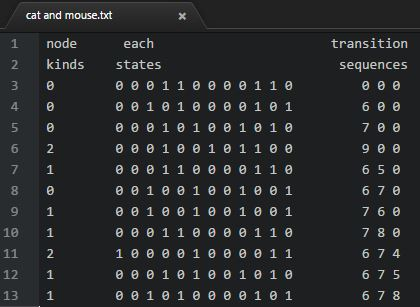
\includegraphics[width=11cm,height=8cm]
	{resultsofcatandmousetxt.JPG}
	
	Figure 5 Result of Program.
	\end{center}
\end{flushleft}
\end{document}